\documentclass{TDP005mall}



\newcommand{\version}{Version 0.1}
\author{Niklas Åsberg, \url{nikas214@student.liu.se}}
\title{Kravspec}
\date{2023-11-12}
\rhead{Niklas Åsberg}
\usepackage{graphicx}
\graphicspath{{./}}


\begin{document}
\projectpage
\section{Revisionshistorik}
\begin{table}[!h]
\begin{tabularx}{\linewidth}{|l|X|l|}
\hline
Ver. & Revisionsbeskrivning & Datum \\\hline
0.1 & Utkast & 2023-11-12 \\\hline
\end{tabularx}
\end{table}

\tableofcontents
\newpage

\section{Spelidé}
Spelet är ett tvådimentionellt arkadspel, målet är att ta sig igenom så många labyrinter som möjligt på så kort tid som möjligt utan att dö.
Spelplanen är ett rutnät, all förflyttning sker mellan rutor intill varandra. Det kommer finnas väggar på vissa rutor som man inte kan röra sig igenom.
Det kommer vara massa fiender ivägen för spelaren som spelaren ska ta sig förbi eller förinta. Fiender kan skada spelaren om de hamnar i samma ruta, hur mycket skada spearen tar är olika beroende på fiende-typ
Spelaren kan attackera fiender när fienderna är en ruta bort.

\section{Målgrupp}
Målgruppen för spelet är de som gillar arkadspel och speed-runners.

\section{Spelupplevelse}
Spelet har mycket fokus på snabbhet, så spelaren kommer att försöka slå sin bästa tid och tävla med andra spelara om vem som får högst poäng.

\section{Spelmekanik}
Man styr sin spelare med W, A, S och D tangenterna och attackerar med mellanslag. Varje bana är en labyrint när spelaren ska ta sig till utgången, när spelaren tagit sig till utgången så börjar nästa bana.
Det finns fiender som är i vägen och dessa kommer att skada spelaren om de är på samma ruta.
Spelaren behöver inte nödvändigtvis förinta fienderna för att klara banan men spelaren får extrapoäng om spelaren förintar fiender.

\section{Regler}
Varken spelaren eller fiender kan röra sig till en ruta där det finns en vägg.
Spelaren tar skada om spelaren befinner sig på samma ruta som en fiende.
Spelaren kan skada en fiende genom att attackera.
När spelaren är på rutan där utgången finns så flyttas spelaren till nästa bana.
Om spelaren inte har några livspoäng kvar så börjar spelet om.
Spelaren "Vinner" genom att ta sig igenom alla banor.

\newpage
\section{Visualisering}
Spelet kommer vara tvådimentionellt och vara ur ett fågelperspektiv.

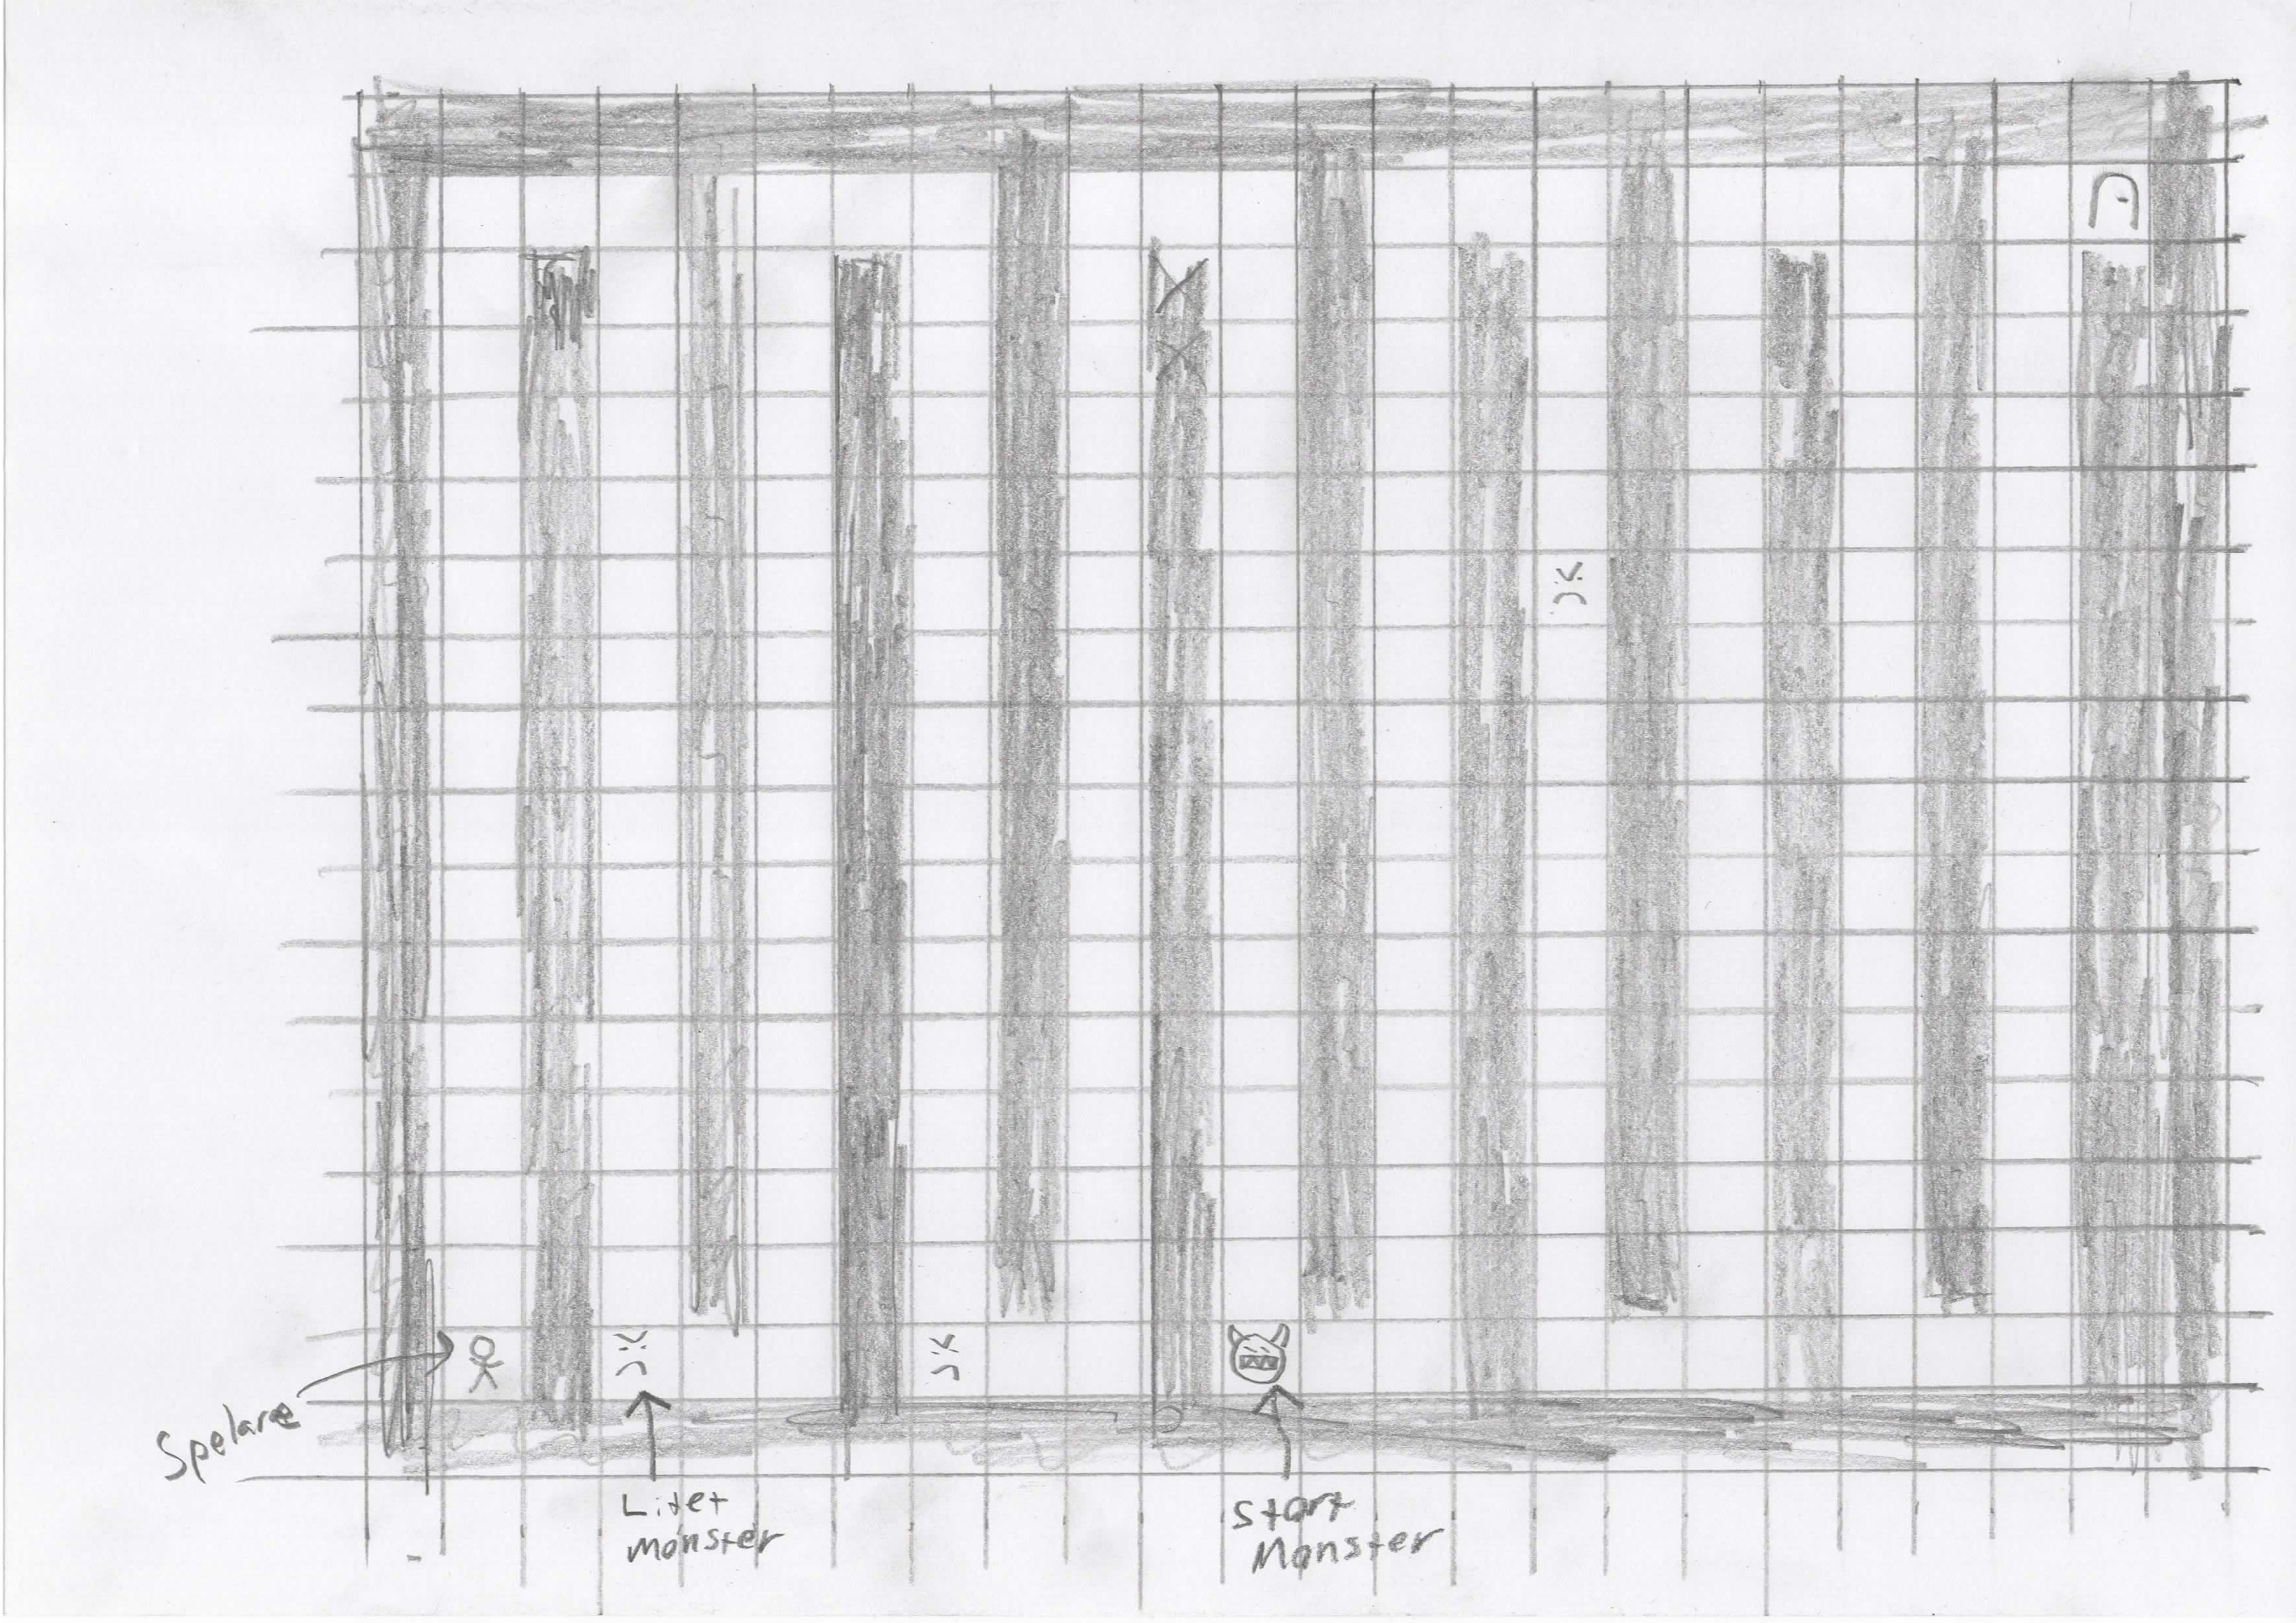
\includegraphics[scale=0.5]{Spelskiss}

\newpage
\section{Kravformulering}
\subsection{Ska-krav}
\begin{enumerate}
  \item Spelplanen ska vara ett rutnät där rörelse sker från en ruta till en annan
  \item Spelplanen ska vara en labyrint
  \item Väggar ska finnas på vissa rutor
  \item Spelaren ska kunna röra sig åt fyra håll med hjälp av W, A, S och D
  \item Spelaren ska inte kunna gå på en ruta där det finns en vägg
  \item När spelaren trycker på mellanslag ska spelaren attackera
  \item Fiender ska röra sig mellan rutor enligt en fördefinerad bana
  \item Fiender ska skada spelaren när de är på samma ruta
  \item 2 typer av fiender ska finnas, en stor och en liten
  \item Det ska finnas en ruta som är utgången
  \item Om spelaren står på rutan med utgången ska näsa bana påbörjas
  \item Poängen ska räknas baserat på antalet förintade fiender och tiden det tar att klara spelet
\end{enumerate}

\subsection{Bör-krav}
\begin{enumerate}
  \item Fiender ska ha en chans att släppa ett liv när de förintas
  \item Spelare ska kunna plocka upp liv för att fylla på sin hälsa
  \item Fienderna ska röra sig mot spelaren när spelaren är inom synhåll
\end{enumerate}

\newpage
\section{Kravuppfyllelse}


\textbf{Spelet ska simulera en värld som innehåller olika typer av objekt. Objekten ska ha olika beteenden och röra sig i världen och agera på olika sätt när de möter andra objekt.}

Uppfylls av krav 1, 2, 5, 8 och 11.

\textbf{Det måste finnas minst tre olika typer av objekt och det ska finnas flera instanser av minst två av dessa. T.ex ett spelarobjekt och många instanser av två olika slags fiendeobjekt.}

Det finns en spelare och två typer av fiender, en stor och en liten.

\textbf{Ett beteende som måste finnas med är att figurerna ska röra sig över skärmen. Rörelsen kan följa ett mönster och/eller vara slumpmässig. Minst ett objekt, utöver spelaren ska ha någon typ av rörelse.}

Både spelaren och båda fienderna kommer röra sig över spelplanen.

\textbf{En figur ska styras av spelaren, antingen med tangentbordet eller med musen. Du kan även göra ett spel där man spelar två stycken genom att dela på tangentbordet (varje spelare använder olika tangenter). Då styr man var sin figur.}

Spelaren styrs av W, A, S och D tangenterna och kan attackera med mellanslag.

\textbf{Grafiken ska vara tvådimensionell.}

Grafiken kommer vara tvådimensionell

\textbf{Världen (spelplanen) kan antas vara lika stor som fönstret (du kan göra en större spelplan med scrollning, men det blir lite krångligare).}

Labyrinten kommer fylla fönstret, när nästa bana påbörjas så kommer den nya labyrinten  att ersätta den den gamla.

\textbf{Det ska finnas kollisionshantering, det vill säga, det ska hända olika saker när objekten möter varandra, de ska påverka varandra på något sätt. T.ex kan ett av objekten tas bort, eller så kan objekten förvandlas på något sätt, eller så kan ett nytt objekt skapas. (Ett exempel på att skapa/ta bort objekt är när man i Space Invaders trycker på skjuta-knappen, t.ex en musknapp, då avfyras ett laserskott och skottet blir då en ny figur som skapas och placeras i världen, på en position vid laserkanonens mynning. Skottet rör sig framåt (uppåt) och om det träffar ett fiendeskepp tas både skottet och skeppet bort, om skottet kommer utanför spelplanen, dvs det missar, tas det endast bort.)}

Spelaren kommer ta skada om den koliderar med en fiende.



\end{document}
